\documentclass[12pt,addpoints]{exam}
\usepackage{enumitem}
\usepackage{amsfonts,amssymb,amsmath, amsthm}
\usepackage{graphicx}
\usepackage{systeme}
\usepackage{pgf,tikz,pgfplots}
\pgfplotsset{compat=1.15}
\usepgfplotslibrary{fillbetween}
\usepackage{mathrsfs}
\usetikzlibrary{arrows}
\usetikzlibrary{calc}
\usepackage{geometry}
\geometry{
	a4paper,
	total={170mm,257mm},
	left=15mm,
	right=15mm,
	bottom=20mm,
	top=15mm,
}
\date{December, 2023}
\pagestyle{headandfoot}
%\firstpageheadrule
\runningheader{}{}{Page \thepage\ of \numpages}
\runningheadrule
\firstpagefooter{}{}{}
\runningfooter{The latex group}{}{Page \thepage\ of \numpages}
\begin{document}
	\title{St John Baptist De La Salle Catholic School, Addis Ababa\\
		\large Grade 11 ESSLCE Physics Prep Questions\\
		\author{The latex group}
		$2^\text{nd}$ Quarter}
	\maketitle
	\subsection*{Multiple Choice Questions}
	\begin{questions}
		\question The diagram shown below is a velocity-time graph for a car moving in a straight line. What is the displacement of the car after 10s? \\
		\begin{center}
			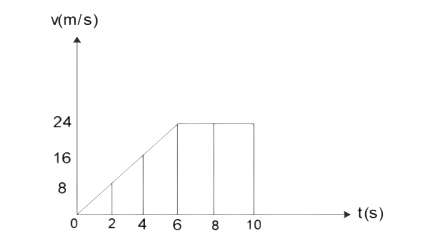
\includegraphics[scale=0.5]{g1.png}
		\end{center}
		\begin{oneparchoices}
			\choice 96m
			\choice 72m
			\choice 240m
			\choice 168m
		\end{oneparchoices}
		\question If a stone is thrown directly downward from the top of a 40m tall building with an initial speed of 10m/s. What will be the speed of the stone when it reaches the ground?($g=10m/s^2,$ \text{air resistance is negligible})\\
		\begin{oneparchoices}
			\choice 40m/s
			\choice 30m/s
			\choice 90m/s
			\choice 50m/s
		\end{oneparchoices}
		\question Which of the following statement is correct? \\
		\begin{choices}
			\choice It is not necessary to consider a reference frame to measure velocity.
			\choice There is a universal reference frame
			\choice Velocity is always measured relative to a reference frame.
			\choice Velocity is independent of a reference frame.
		\end{choices}
		\question Consider a particle performing a circular motion around a circle of radius r, with an angular velocity $\omega$ and the particle's projection on the horizontal diameter of the circle (between points Q and R) as shown in the figure below 
		\begin{center}
			\includegraphics[scale=0.5]{g.png}
		\end{center}
		Which of the following statements is correct about the motion of the particle and its projection on $\overline{QR}$\\
		\begin{choices}
			\choice The projection of the particle on $\overline{QR}$ swings between points Q and R with constant speed.
			\choice The circular motion of particle can be taken as a simple harmonic motion.
			\choice The projection of the particle on $\overline{QR}$ demonstrates simple harmonic motion.
			\choice The projection of the particle on $\overline{QR}$ demonstrates motionwith constant acceleration.
		\end{choices}
		\question Which one of the following groups of physical quantities contains only vectors?\\
		\begin{choices}
			\choice Work, Electric field, Displacement and Force
			\choice Acceleration, Speed, Force and Electric field
			\choice Momentum, Energy, Magnetic field and Force
			\choice Displacement, Velocity, Magnetic field and Momentum
		\end{choices}
		\question Which rule about the number of significant figures is correct? Zeros in the number\\
		\begin{choices}
			\choice 450.0 are significant figures.
			\choice 0.0023 are significant figures.
			\choice 1.1000 are significant figures.
			\choice 2.70018 are significant figures.
		\end{choices}
		\question Given two vectors $v_1=10 units$ aling the positive y-axisand $v_2=6 units$ at an angle of $37^{\circ}$ above the positive x-axis. What is the scalar product of the vectors in square of units?\\
		\begin{oneparchoices}
			\choice 45
			\choice 36
			\choice 48
			\choice 60
		\end{oneparchoices}
		\question An airplane takes-off at airport A and travels 500km due east within one hour and then turning to south it flies for 20 minutes to land on airport B which is 100km away from turning point. The magnitude average velocity of the plane during its flight between two airports is  \\ 
		\begin{oneparchoices}
			\choice 75$\sqrt{24}$ km/hr
			\choice 100$\sqrt{34}$ km/hr
			\choice 450 km/hr
			\choice 75$\sqrt{26}$ km/hr
		\end{oneparchoices}
		\question A bullet is fired with an initial speed v at an angle $\theta$ with the horizontal. It takes a time T to reach its maximum vertical displacement $h_\text{max}$. It hits the target point a distance R away and exactly in the horizontal level to the point where it was fired. Which one of the following statement is \textbf{NOT} correct about the motion of bullet?  \\ 
		\begin{choices}
			\choice The bullet hits the target at a time 2T after it was fired.
			\choice $h_\text{max}$ is directly proportional to the initial speed v.
			\choice R will be maximum if cos$\theta$=$\sqrt{2}/2$.
			\choice $\theta$ should be different from $90^{\circ}$ to hit the target at a distance R.
		\end{choices}
		\question A man pushes a 25.0kg object by 250N force along an inclined plane inclined at an angle of $37^{\circ}$ to the horizontal. If the object moves with constant speed, the friction force exerted on the block is  \\ 
		\begin{choices}
			\choice 250.0 N, up the inclined plane.
			\choice 100.0 N, up the inclined plane.
			\choice 100.0 N, down the inclined plane.
			\choice 250.0 N, down the inclined plane.
		\end{choices}
		\question The following three collisions occur in different systems. \newline
		\begin{enumerate}[label=\Roman*]
			\item A billiard ball A collides with an identical ball B and comes to rest after collision, while ball B moves with the same velocity as ball A was moving before.
			\item A bullet moving with speed v hits a suspended mass and it embedded in it and the combination moves with common velocity.
			\item Two cars moving in opposite direction become at rest after collision.\newline Which of the following statements is correct about these collisions?
		\end{enumerate}
		\begin{choices}
			\choice II and III are inelastic collisons.
			\choice I and II are elastic collisons.
			\choice I, II and III are inelastic collisions.
			\choice I and III are elastic collisions.
		\end{choices}
		\question An object of mass M is attached to a spring of spring constant K, as shown in figure below.
		\begin{center}
		%	\includegraphics[scale=0.5]{g.png}
		\end{center} 
		If the mass is pulled to a point P, which is the distance Afrom equilibrium position O, and released. Which one of the following statements is correct about energy of the system?(\text{assume the surface is frictionless}) \\
		\begin{choices}
			\choice At point O, the system has both kinetic and potential energy.
			\choice At point P, the systemm has both kinetic and potential energy.
			\choice At point P, the mass attain its maximum velocity.
			\choice At point Q the system has both kinetic energy and potential energy.
		\end{choices}
		\question A force $\vec{F}$ = $(\hat{i}-3\hat{k})$ N acts on a wooden bar and drags the bar through a displacement of $\vec{r}$ = $4-\hat{i}m$. WHat is the torque due to the force N.m?  \\ 
		\begin{oneparchoices}
			\choice $4\hat{i}+12\hat{j}$
			\choice $-12\hat{j}$
			\choice $12\hat{j}$
			\choice $12\hat{k}$
		\end{oneparchoices}
		\question Consider a system of two point masses $M_1$ and $M_2$ with $M_1 = 0.5$ $M_2$. The two masses are located on the x-y plane as shown in the figure below. 
		\begin{center}
			\includegraphics[scale=0.5]{g.png}
		\end{center} 
		Which one of the following alternatives indicates the position of center of mass of the systems? \\
		\begin{oneparchoices}
			\choice(5/3,7/3)cm
			\choice (5,4)cm
			\choice(11/3,16/3)cm
			\choice (16/3,11/3)cm
		\end{oneparchoices}
		\question Which one of the following is correct about mechanica waves? \\
		\begin{choices}
			\choice The number of complete waves passes a given point per time is called the period of teh waves.
			\choice The distance between two identical points on adjacent points on adjacent waves is known as the wavelength of the wave.
			\choice The time taekn for one complete wave to pass a given point is called the frequency of the wave.
			\choice The maximum height in a transverse wave is known as the trough of the wave.
		\end{choices}
		\question A boy in a journey covers his route by traveling 3.0 km east and 4.0 north. What is teh magnitude of his resultant displacemnt?
		\begin{center}
		%	\includegraphics[scale=0.5]{g.png}
		\end{center} 
		Which one of the following alternatives indicates the position of center of mass of the systems? \\
		\begin{oneparchoices}
			\choice 2.7km
			\choice 7.0km
			\choice 1.0km
			\choice 5.0km
		\end{oneparchoices}
		\question The graph below shows the velocity of a man travelling on a motorcycle as a function of time
		\begin{center}
			\includegraphics[scale0.5]{g.png}
		\end{center}
		Which one of the following statements is correct aabout the velocity-time graph? \\
		\begin{choices}
			\choice The acceleration in the first 6 is equal to the gradient of the curve in the given interval and it is positive.
			\choice The acceleration during the time interval from $t=6s$ to $t=10s$ is equal to the gradient of the curve in the given interval and it is negative.
			\choice The dispacement during te time intervals $t=0s$ to $t=6s$ is equal to the area under the velocity-time graph in the given interval
			\choice The displacement during the time. interval from $t=6s$ to $t=14s$ is equal to the area of region II minus the area of region III.
		\end{choices}
	\end{questions}
\end{document}
